\documentclass[english,man]{apa6}

\usepackage{amssymb,amsmath}
\usepackage{ifxetex,ifluatex}
\usepackage{fixltx2e} % provides \textsubscript
\ifnum 0\ifxetex 1\fi\ifluatex 1\fi=0 % if pdftex
  \usepackage[T1]{fontenc}
  \usepackage[utf8]{inputenc}
\else % if luatex or xelatex
  \ifxetex
    \usepackage{mathspec}
    \usepackage{xltxtra,xunicode}
  \else
    \usepackage{fontspec}
  \fi
  \defaultfontfeatures{Mapping=tex-text,Scale=MatchLowercase}
  \newcommand{\euro}{€}
\fi
% use upquote if available, for straight quotes in verbatim environments
\IfFileExists{upquote.sty}{\usepackage{upquote}}{}
% use microtype if available
\IfFileExists{microtype.sty}{\usepackage{microtype}}{}

% Table formatting
\usepackage{longtable, booktabs}
\usepackage{lscape}
% \usepackage[counterclockwise]{rotating}   % Landscape page setup for large tables
\usepackage{multirow}		% Table styling
\usepackage{tabularx}		% Control Column width
\usepackage[flushleft]{threeparttable}	% Allows for three part tables with a specified notes section
\usepackage{threeparttablex}            % Lets threeparttable work with longtable

% Create new environments so endfloat can handle them
% \newenvironment{ltable}
%   {\begin{landscape}\begin{center}\begin{threeparttable}}
%   {\end{threeparttable}\end{center}\end{landscape}}

\newenvironment{lltable}
  {\begin{landscape}\begin{center}\begin{ThreePartTable}}
  {\end{ThreePartTable}\end{center}\end{landscape}}

  \usepackage{ifthen} % Only add declarations when endfloat package is loaded
  \ifthenelse{\equal{\string man}{\string man}}{%
   \DeclareDelayedFloatFlavor{ThreePartTable}{table} % Make endfloat play with longtable
   % \DeclareDelayedFloatFlavor{ltable}{table} % Make endfloat play with lscape
   \DeclareDelayedFloatFlavor{lltable}{table} % Make endfloat play with lscape & longtable
  }{}%



% The following enables adjusting longtable caption width to table width
% Solution found at http://golatex.de/longtable-mit-caption-so-breit-wie-die-tabelle-t15767.html
\makeatletter
\newcommand\LastLTentrywidth{1em}
\newlength\longtablewidth
\setlength{\longtablewidth}{1in}
\newcommand\getlongtablewidth{%
 \begingroup
  \ifcsname LT@\roman{LT@tables}\endcsname
  \global\longtablewidth=0pt
  \renewcommand\LT@entry[2]{\global\advance\longtablewidth by ##2\relax\gdef\LastLTentrywidth{##2}}%
  \@nameuse{LT@\roman{LT@tables}}%
  \fi
\endgroup}


  \usepackage{graphicx}
  \makeatletter
  \def\maxwidth{\ifdim\Gin@nat@width>\linewidth\linewidth\else\Gin@nat@width\fi}
  \def\maxheight{\ifdim\Gin@nat@height>\textheight\textheight\else\Gin@nat@height\fi}
  \makeatother
  % Scale images if necessary, so that they will not overflow the page
  % margins by default, and it is still possible to overwrite the defaults
  % using explicit options in \includegraphics[width, height, ...]{}
  \setkeys{Gin}{width=\maxwidth,height=\maxheight,keepaspectratio}
\ifxetex
  \usepackage[setpagesize=false, % page size defined by xetex
              unicode=false, % unicode breaks when used with xetex
              xetex]{hyperref}
\else
  \usepackage[unicode=true]{hyperref}
\fi
\hypersetup{breaklinks=true,
            pdfauthor={},
            pdftitle={Using Beta Regression to Model Normative Aspects of Prejudice and Political Attitudes: With Applications in R},
            colorlinks=true,
            citecolor=blue,
            urlcolor=blue,
            linkcolor=black,
            pdfborder={0 0 0}}
\urlstyle{same}  % don't use monospace font for urls

\setlength{\parindent}{0pt}
%\setlength{\parskip}{0pt plus 0pt minus 0pt}

\setlength{\emergencystretch}{3em}  % prevent overfull lines

\ifxetex
  \usepackage{polyglossia}
  \setmainlanguage{}
\else
  \usepackage[english]{babel}
\fi

% Manuscript styling
\captionsetup{font=singlespacing,justification=justified}
\usepackage{csquotes}
\usepackage{upgreek}



\usepackage{tikz} % Variable definition to generate author note

% fix for \tightlist problem in pandoc 1.14
\providecommand{\tightlist}{%
  \setlength{\itemsep}{0pt}\setlength{\parskip}{0pt}}

% Essential manuscript parts
  \title{Using Beta Regression to Model Normative Aspects of Prejudice and
Political Attitudes: With Applications in R}

  \shorttitle{Beta Regression}


  \author{Mark H. White II\textsuperscript{1}}

  \def\affdep{{""}}%
  \def\affcity{{""}}%

  \affiliation{
    \vspace{0.5cm}
          \textsuperscript{1} University of Kansas  }

  \authornote{
    \newcounter{author}
    Author note will go here.

                      Correspondence concerning this article should be addressed to Mark H. White II. E-mail: \href{mailto:markhwhiteii@gmail.com}{\nolinkurl{markhwhiteii@gmail.com}}
                }


  \abstract{Abstract will go here.}
  \keywords{beta regression, hurdle models, gamlss, norms, social attitudes \\

    
  }





\usepackage{amsthm}
\newtheorem{theorem}{Theorem}
\newtheorem{lemma}{Lemma}
\theoremstyle{definition}
\newtheorem{definition}{Definition}
\newtheorem{corollary}{Corollary}
\newtheorem{proposition}{Proposition}
\theoremstyle{definition}
\newtheorem{example}{Example}
\theoremstyle{remark}
\newtheorem*{remark}{Remark}
\begin{document}

\maketitle

\setcounter{secnumdepth}{0}



\section{Statistical Background}\label{statistical-background}

\subsection{The Beta Distribution}\label{the-beta-distribution}

The beta distribution can be used in a generalized linear model when the
values of the dependent variable are bounded \(0 < y < 1\) (Coxe, West,
\& Aiken, 2013). The probability density function (pdf) of the beta
distribution is determined by two parameters, \(\alpha\) and \(\beta\),
that are called \enquote{shape} parameters:

\begin{center}
$f(y;\alpha,\beta)={\Gamma(\alpha+\beta)\over\Gamma(\alpha)\Gamma(\beta)}y^{\alpha-1}(1-y)^{\beta-1}$
\end{center}

where \(\Gamma(.)\) is the gamma function. One of the benefits of the
beta distribution is that it is flexible and can take a number of
distributional shapes (Figure 1).

\begin{figure}
\centering
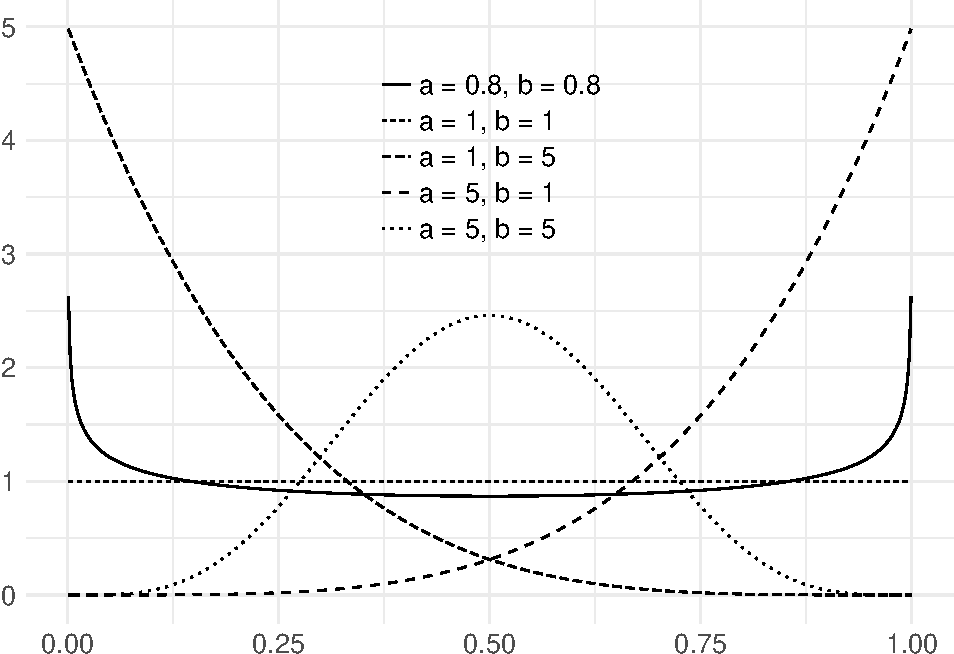
\includegraphics{beta_hurdle_files/figure-latex/unnamed-chunk-2-1.pdf}
\caption{\label{fig:unnamed-chunk-2}Beta probability density functions with
various combinations of shape parameters.}
\end{figure}

These parameters are not inherently meaningful to researchers, however.
Rigby, Stasinopoulos, Heller, and De Bastiani (2017)
\enquote{reparameterized} the beta distribution so that the two
parameters determining the shape of the distribution would be more
useful in a regression framework (but see Ferrari \& Cribari-Neto, 2004
for a different parameterization). Instead of predicting \(\alpha\) and
\(\beta\), they parameterize (i.e., algebraically rearrange parameters)
so that beta regression predicts two different parameters: \(\mu\)
(called the \enquote{location} parameter) and \(\sigma\) (called the
\enquote{scale} parameter), where \(\mu={\alpha\over(\alpha+\beta)}\)
and \(\sigma=\sqrt{1\over(\alpha+\beta+1)}\). \(\mu\) is equivalent to
the mean, and \(\sigma\) is related positively to the variance (note
that \(\sigma\) is \emph{not} the standard deviation, even though
\(\sigma\) commonly refers to the standard deviation). The variance is
equivalent to \(\sigma^2\mu(1-\mu)\), and there are two things to note
from this equation: First, the greater the \(\sigma\), the greater the
variance; second, the variance depends on the mean, which means that
beta regression will be naturally heteroskedastic (covered shortly).
Using this distribution in a regression framework cannot handle the
dependent variable taking on values 0 and 1---how can we model dependent
variables in the range \(0 \leq y \leq 1\)?

\subsection{Zero-One Inflated Beta
Distribution}\label{zero-one-inflated-beta-distribution}

Rigby et al. (2017) show that the beta distribution can be
\enquote{inflated} at 0 and 1, meaning the dependent variable contains
0s and 1s (i.e., \(0 \leq y \leq 1\)), the pdf for this beta inflated
distribution, \(\text{beinf}\), is:

\begin{center}
\[
\text{beinf}(y;\mu,\sigma,\nu,\tau) =
\begin{cases}
  p_0                             & \text{if } y = 0\\
  (1 - p_0 - p_1)f(y;\mu,\sigma)  & \text{if } 0 < y < 1\\
  p_1                             & \text{if } y = 1
\end{cases}
\]
\end{center}

for \(0 \leq y \leq 1\), where \(f(y;\mu,\sigma)\) is the beta pdf with
\(\mu\) and \(\sigma\) bounded \emph{between} zero and one. The two
additional parameters, \(\nu\) and \(\tau\), are related to \(p_0\) and
\(p_1\), respectively. \(p_0\) is the probability that a case equals
zero, \(p_1\) is the probability that a case equals one, and \(p_2\)
(i.e., \(1 - p_0 - p_1\)) is the probability that the case comes from
the beta distribution. In terms of these two additional parameters,
\(p_0 = {\nu \over (1 + \nu + \tau)}\) and
\(p_1 = {\tau \over (1 + \nu + \tau)}\). Rearranging these
algebraically, \(\nu\) is the odds that a case is 0 to being
\(0 < y < 1\), \(\nu = p_0 / p_2\), and \(\tau\) is the odds that a case
is a 1 to being \(0 < y < 1\), \(\tau = p_1 / p_2\).

\subsection{Beta Regression Models}\label{beta-regression-models}

The goal for a researcher now is to predict these four parameters,
\(\mu, \sigma, \nu, \tau\), from any number of predictor variables of
theoretical interest. All four parameters can be predicted by an
identical set of predictors, none of the same predictors, or any
mixture. Both \(\mu\) and \(\sigma\) have to be between zero and one
(since the beta distribution is bounded between 0 and 1), so one can use
the logistic link function to fit predicted values in this range. Both
\(\nu\) and \(\tau\) have to be greater than zero (since they are odds),
so one can use the log link function to fit predicted values in this
range. Imagine a researcher has one predictor of interest, \(x\). They
could include this variable as a predictor of all four variables with
the equations:

\begin{center}
$\text{log}({\mu \over 1 - \mu}) = \beta_{10} + \beta_{11}X$\\
$\text{log}({\sigma \over 1 - \sigma}) = \beta_{20} + \beta_{21}X$\\
$\text{log}(\nu) = \beta_{30} + \beta_{31}X$\\
$\text{log}(\tau) = \beta_{40} + \beta_{41}X$
\end{center}

Or equivalently:

\begin{center}
$\mu={1\over1+e^{-(\beta_{10}+\beta_{11}X)}}$\\
$\sigma={1\over1+e^{-(\beta_{20}+\beta_{21}X)}}$\\
$\nu = e^{\beta_{30} + \beta_{31}X}$\\
$\tau = e^{\beta_{40} + \beta_{41}X}$
\end{center}

where \(e^x\) is the natural exponential function. A different inflated
beta distribution can also be used when the dependent variable contains
0s but not 1s (e.g., \(0 \leq y < 1\)) or when it contains 1s but not 0s
(e.g., \(0 < y \leq 1\)). Let \(c\) be the value---0 or 1---that is
included (i.e., inflated). The pdf is:

\begin{center}
\[
\text{beinf}_c(y;\mu,\sigma,\nu) =
\begin{cases}
  p_c                             & \text{if } y = c\\
  (1 - p_c)f(y;\mu,\sigma)        & \text{if } 0 < y < 1\\
\end{cases}
\]
\end{center}

where \(\nu = p_c / (1 - p_c)\) and the remaining notation is the same
as in the zero-and-one inflated beta distribution. The same link
functions are used, but the fourth parameter, \(\tau\), is not included,
since the distribution is only inflated at \(c\). Lastly, if no 0s or 1s
are observed, the beta distribution alone can be used as the pdf. This
results in a beta regression where the researcher is only predicting the
location, \(\mu\), and shape, \(\sigma\). Since there is no inflation at
0 or 1, the latter two parameters, \(\nu\) and \(\tau\), are not
included.

\subsection{Modeling Bounded Variables Beyond the Zero Through One
Range}\label{modeling-bounded-variables-beyond-the-zero-through-one-range}

These beta regression models are commonly used when rates and
proportions are dependent variables, given that these are naturally
bounded \(0 \leq y \leq 1\) (Buntaine, 2011; Eskelson, Madsen, Hagar, \&
Temesgen, 2011; Gallardo, Bovea, Colomer, \& Prades, 2012; Hubben et
al., 2008; Peplonska et al., 2012). More generally, however, the beta
distribution is a doubly bounded continuous distribution: Although it is
on a continuous scale, values cannot be exceed the upper bound, \(u\),
or be less than the lower bound, \(l\). In the case of the zero-and-one
inflated beta distribution, \(l = 0\) and \(u = 1\).

Most scales used to measure prejudice and political attitudes are doubly
bounded and continuous. Although researchers generally model variables
on Likert scales and sliding scales (e.g., feeling thermometers) as
being conditionally normally distributed (i.e., using ordinary least
squares regression), these variables are not strictly normal.
Observations from a normal distribution can take on any value on the
real number line, while observations from a standard 7-point Likert
scale can only take on values 1 through 7---and in studying
controversial and polarizing issues like prejudice and politics, many
participants score at the lower or upper bounds, causing floor or
ceiling effects. In these cases, the assumptions of normality and
homoskedasticity are likely to be violated. Many times researchers
create, update, or seek out measures to so that the distributional form
of the dependent variable takes on a normal shape---statistical
assumptions are directing the phenomenon researchers choose to observe
and the theoretical questions that they ask. Instead, one can explicitly
take into account that the response is doubly bounded and
heteroskedastic by using the beta regression models described above,
using a simple linear rescaling of the data.

If one observes a dependent variable limited between two bounds, there
is a straightforward way to rescale the variable to the
\(0 \leq y \leq 1\) range:

\begin{center}
$y'_i = (y_i - l) / (u - l)$
\end{center}

where \(y\) is the variable on the original scale, \(y'\) is the
rescaled variable, \(u\) is the upper bound (i.e., the largest possible
value on the scale), \(l\) is the lower bound (i.e., the smallest
possible value on the scale), and the \(i\) subscript denotes an
individual's score. On a standard 7-point Likert scale, \(l = 1\) and
\(u = 7\). This rescaling allows a researcher to explicitly model
conditional variance, floor effects, and ceiling effects using beta
regression.

\subsubsection{Conditional variance}\label{conditional-variance}

Observing a dependent variable that is doubly bounded and continuous can
produce heteroskedasticity. One of the assumptions of an OLS regression
is homoskedasticity---that the variance of the errors are unrelated to
any predictor, any linear combination of predictors, and the predicted
values. A regression equation with one predictor variable \(x\) is often
written as \(y_i = \beta_0 + \beta_1x_i + \epsilon_i\), where
\(\epsilon_i\) is how far an osbserved value \(y_i\) is from the
predicted value (i.e., the residual). Let \(\hat{y_i}\) be the predicted
value for observation \(i\), where \(\hat{y_i} = \beta_0 + \beta_1x_i\).
We can simplify the equation to \(y_i = \hat{y_i} + \epsilon_i\), where
the residuals \(\epsilon\) are normally distributed with a mean of 0 and
some variance---that is, \(\epsilon \sim N(0, \sigma^2_\epsilon)\). We
can further simplify this to:
\(y_i|x_i \sim N(\hat{y_i}, \sigma^2_\epsilon)\), which means that each
observation of the dependent variable we make, given the predictors we
use, is normally distributed with a mean of that observation's predicted
score and some variance. The assumption of homoskedasticity is found in
that \(\sigma^2_\epsilon\) does \emph{not} have a subscript \(i\). This
means that there is one \emph{common variance} of the residuals.

Imagine one runs a regression and observes
\(\hat{y_i} = 2.5 + 1.5 \times x_i\) and \(\sigma^2_\epsilon = 9\). Say
that the first individual's score on \(x\) is 0, \(x_1 = 0\), and the
second individual's score is \(x_2 = 5\). The model then assumes that
the first person comes from a normal distribution with a mean of 4
(i.e., \(\hat{y_1}\)) and a variance of 9 (i.e., \(\sigma^2_\epsilon\)),
while the second person comes from a normal distribution with a mean of
10 and that same variance of 9. The violation of this assumption can
lead to inflated Type I errors or diminished statistical power,
depending on the type and source of the heteroskedasticity (Hayes \&
Cai, 2007; Long \& Ervin, 2000; Rosopa, Schaffer, \& Schroeder, 2013).

While common remedies for heteroskedasticity (e.g., robust standard
errors, transforming the dependent variable, weighted least squares)
treat it as a nuisance to be corrected for when calculating \(p\)-values
(Hayes \& Cai, 2007; Long \& Ervin, 2000; Rosopa et al., 2013), it could
be that explicitly modeling this conditional variance is an interesting
phenomenon per se. Heteroskedasticity can arise when the error variance
is predicted by one of the observed predictor variables, and since beta
regression models predict a shape parameter, \(\sigma\), a researcher
can explicitly model this relationship. This allows researchers to ask
questions about conditional variance: \enquote{Does the variance in
\(y\) increase as \(x\) also increases}? Since the focus of OLS
regression is the \emph{location} parameter (e.g., conditional mean),
researchers might be ignoring interesting, potentially
theoretically-relevant parts of their data. After discussing floor and
ceiling effects, I will argue that normative influences are one of these
aspects.

\subsubsection{Floor and ceiling
effects}\label{floor-and-ceiling-effects}

Floor and ceiling effects occur when there are many observations at the
lower and upper bound of the scale, respectively (Everitt \& Skrondal,
2010). Variables displaying these effects are likely to violate numerous
assumptions of ordinary least squares regression, such as conditional
normality and homoskedasticity of variance. Variables displaying these
effects can be thought of as being censored or truncated; a common
regression technique for censored or truncated variables are Tobit
models (Smithson \& Merkle, 2013). Censoring occurs when all scores
beyond some threshold are recorded at that threshold. If a researcher is
measuring reaction times, censoring occurs if, for example, the
researcher decides that any times above five seconds are scored as five.
If many people score above five, this censoring can cause a ceiling
effect. Truncating occurs when people who score beyond some treshold are
excluded from the data. If the researcher simply does not record trials
that take longer than five seconds, then the data are considered to be
truncated. Tobit models can be useful in these situations. However,
standard Tobit models assume that the underlying dimension is still
normal. A good application of this is in measuring the abilities of
intelligent children (McBee, 2010). The test may be too easy for the
population, resulting in a ceiling effect. Nonetheless, the ability
being measured is assumed to be normally distributed.

In the realm of prejudice and politics, I argue that it is useful to
\emph{not} think of prejudice as coming from a latent normal
distribution. Instead, people engage in a decision-making process. Using
prejudice as an example, people decide whether or not they are going to
admit to feeling any prejudice (i.e., scoring at the floor or above the
floor); if they decide to admit any prejudice, then they decide how much
to report. As another example: When measuring attitudes toward a
polarizing political figure, people decide whether or not to respond
entirely in the negative (i.e., at the floor), entirely in the positive
(i.e., at the ceiling), or somewhere in between. This could result in a
bimodal distribution, with both ceiling and floor effects.

This decision making process can be modeled with the inflated beta
regression models described above (at zero and one, zero only, or one
only). While these are often referred to as \enquote{zero-one inflated
beta regression} models in papers on beta regression, a more general
name used for these types of models are \enquote{two-part} models (Coxe
et al., 2013); when one assumes a decision-making process behind the two
parts, they are often referred to as \enquote{hurdle} models in the
econometrics literature (Cameron \& Trivedi, 2005; Wooldridge, 2010).

Hurdle models are a generalization of the Type I Tobit model (Cragg,
1971). (But note that, unlike the standard Tobit model, the latent
dependent construct is assumed to be conditionally \emph{beta}
distributed, which can take on many distributional forms, Figure 1.)
They are often used to model count processes with excess zeros (see
Carlevaro, Croissant, \& Hoareau, 2017 for a review of applications).
The log likelihood function for these models can be separated in two
parts: First, a logistic regression modeling the probability of zero
versus greater than zero; second, a truncated negative binomial model
using just the cases with observed dependent values greater than zero.
The inflated beta regressions can be seen as hurdle models, as the
zero-and-one inflated model's log likelihood can also be separated in
two parts: First, a multinomial logistic regression modeling the
probability of observing a zero, one, or a value between zero and one;
Second, a beta regression model using just the cases with observed
values between zero and one. Similarly, The inflated beta regression at
\emph{either} zero \emph{or} one has a log likelihood function that can
be separated in two parts: First, a logistic regression modeling the
probability of observing where the inflation occurs or between zero and
one; Second, a beta regression modeling just the cases with dependent
values between zero and one (Rigby et al., 2017).

Since their likelihoods can be separated, this makes a critical
assumption: That the two processes are independent, given the observed
predictors. In other words, the error terms of each submodel are assumed
to be independent of one another. Dependencies between them can be
modeled (referred to as ``selection'' models; Carlevaro et al., 2017;
Wooldridge, 2010), but I will not demonstrate these models here, as they
are not extended to beta regression.

\section{Norms Produce Invariance and Ceiling and Floor
Effects}\label{norms-produce-invariance-and-ceiling-and-floor-effects}

Data from MTurk

\section{Implementation in GAMLSS}\label{implementation-in-gamlss}

Show example from FoRS data

\newpage

\section{References}\label{references}

\setlength{\parindent}{-0.5in} \setlength{\leftskip}{0.5in}

\hypertarget{refs}{}
\hypertarget{ref-buntaine2011does}{}
Buntaine, M. T. (2011). Does the Asian Development Bank respond to past
environmental performance when allocating environmentally risky
financing? \emph{World Development}, \emph{39}(3), 336--350.

\hypertarget{ref-cameron2005microeconometrics}{}
Cameron, A. C., \& Trivedi, P. K. (2005). \emph{Microeconometrics:
Methods and applications}. New York, NY: Cambridge university press.

\hypertarget{ref-carlevaro2016multiple}{}
Carlevaro, F., Croissant, Y., \& Hoareau, S. (2017). \emph{Multiple
hurdle Tobit models in R: The mhurdle package}. Retrieved from
\url{https://cran.r-project.org/web/packages/mhurdle/vignettes/mhurdle.pdf}

\hypertarget{ref-coxe2013generalized}{}
Coxe, S., West, S. G., \& Aiken, L. S. (2013). Generalized linear
models. In T. D. Little (Ed.), \emph{The Oxford handbook of quantitative
methods, volume 2} (pp. 26--51). New York, NY: Oxford University Press.

\hypertarget{ref-cragg1971some}{}
Cragg, J. G. (1971). Some statistical models for limited dependent
variables with application to the demand for durable goods.
\emph{Econometrica: Journal of the Econometric Society}, 829--844.

\hypertarget{ref-eskelson2011estimating}{}
Eskelson, B. N., Madsen, L., Hagar, J. C., \& Temesgen, H. (2011).
Estimating riparian understory vegetation cover with beta regression and
copula models. \emph{Forest Science}, \emph{57}(3), 212--221.

\hypertarget{ref-everitt2002cambridge}{}
Everitt, B., \& Skrondal, A. (2010). \emph{The cambridge dictionary of
statistics}. New York, NY: Cambridge University Press.

\hypertarget{ref-ferrari2004beta}{}
Ferrari, S., \& Cribari-Neto, F. (2004). Beta regression for modelling
rates and proportions. \emph{Journal of Applied Statistics},
\emph{31}(7), 799--815.

\hypertarget{ref-gallardo2012analysis}{}
Gallardo, A., Bovea, M. D., Colomer, F. J., \& Prades, M. (2012).
Analysis of collection systems for sorted household waste in Spain.
\emph{Waste Management}, \emph{32}(9), 1623--1633.

\hypertarget{ref-hayes2007using}{}
Hayes, A. F., \& Cai, L. (2007). Using heteroskedasticity-consistent
standard error estimators in OLS regression: An introduction and
software implementation. \emph{Behavior Research Methods}, \emph{39}(4),
709--722.

\hypertarget{ref-hubben2008societal}{}
Hubben, G. A. A., Bishai, D., Pechlivanoglou, P., Cattelan, A. M.,
Grisetti, R., Facchin, C., \ldots{} Tramarin, A. (2008). The societal
burden of HIV/AIDS in Northern Italy: An analysis of costs and quality
of life. \emph{AIDS Care}, \emph{20}(4), 449--455.

\hypertarget{ref-long2000using}{}
Long, J. S., \& Ervin, L. H. (2000). Using heteroscedasticity consistent
standard errors in the linear regression model. \emph{The American
Statistician}, \emph{54}(3), 217--224.

\hypertarget{ref-mcbee2010modeling}{}
McBee, M. (2010). Modeling outcomes with floor or ceiling effects: An
introduction to the tobit model. \emph{Gifted Child Quarterly},
\emph{54}(4), 314--320.

\hypertarget{ref-peplonska2012rotating}{}
Peplonska, B., Bukowska, A., Sobala, W., Reszka, E., Gromadzińska, J.,
Wasowicz, W., \ldots{} Ursin, G. (2012). Rotating night shift work and
mammographic density. \emph{Cancer, Epidemiology, Biomarkers, \&
Prevention}, \emph{21}(7), 1028--1037.

\hypertarget{ref-rigby2017distributions}{}
Rigby, R., Stasinopoulos, M., Heller, G., \& De Bastiani, F. (2017).
\emph{Distributions for modelling location, scale, and shape: Using
GAMLSS in R. Unpublished draft}. Retrieved from
\url{gamlss.com/books-articles}

\hypertarget{ref-rosopa2013managing}{}
Rosopa, P. J., Schaffer, M. M., \& Schroeder, A. N. (2013). Managing
heteroscedasticity in general linear models. \emph{Psychological
Methods}, \emph{18}(3), 335.

\hypertarget{ref-smithson2013generalized}{}
Smithson, M., \& Merkle, E. C. (2013). \emph{Generalized linear models
for categorical and continuous limited dependent variables}. Boca Raton,
FL: CRC Press.

\hypertarget{ref-wooldridge2010econometric}{}
Wooldridge, J. M. (2010). \emph{Econometric analysis of cross section
and panel data}. Cambridge, MA: MIT press.






\end{document}
